\noindent \textred{2.} 
How many bits are required to encode the message ``aaabccxxxyyyyzz” using Huffman Codes? Please show the coding tree you build. \\
\myAnswer{
First, we need to count the frequency of each character and sort them in ascending order:
\begin{table}[!h]
    \centering
    \begin{tabular}{|c|c|c|c|c|c|}
        \hline
        b & c & z & a & x & y \\
        \hline
        1 & 2 & 2 & 3 & 3 & 4 \\
        \hline
    \end{tabular}
\end{table}
\\
Then we can build the prefix tree accordingly
\begin{figure}[!h]
    \centering
    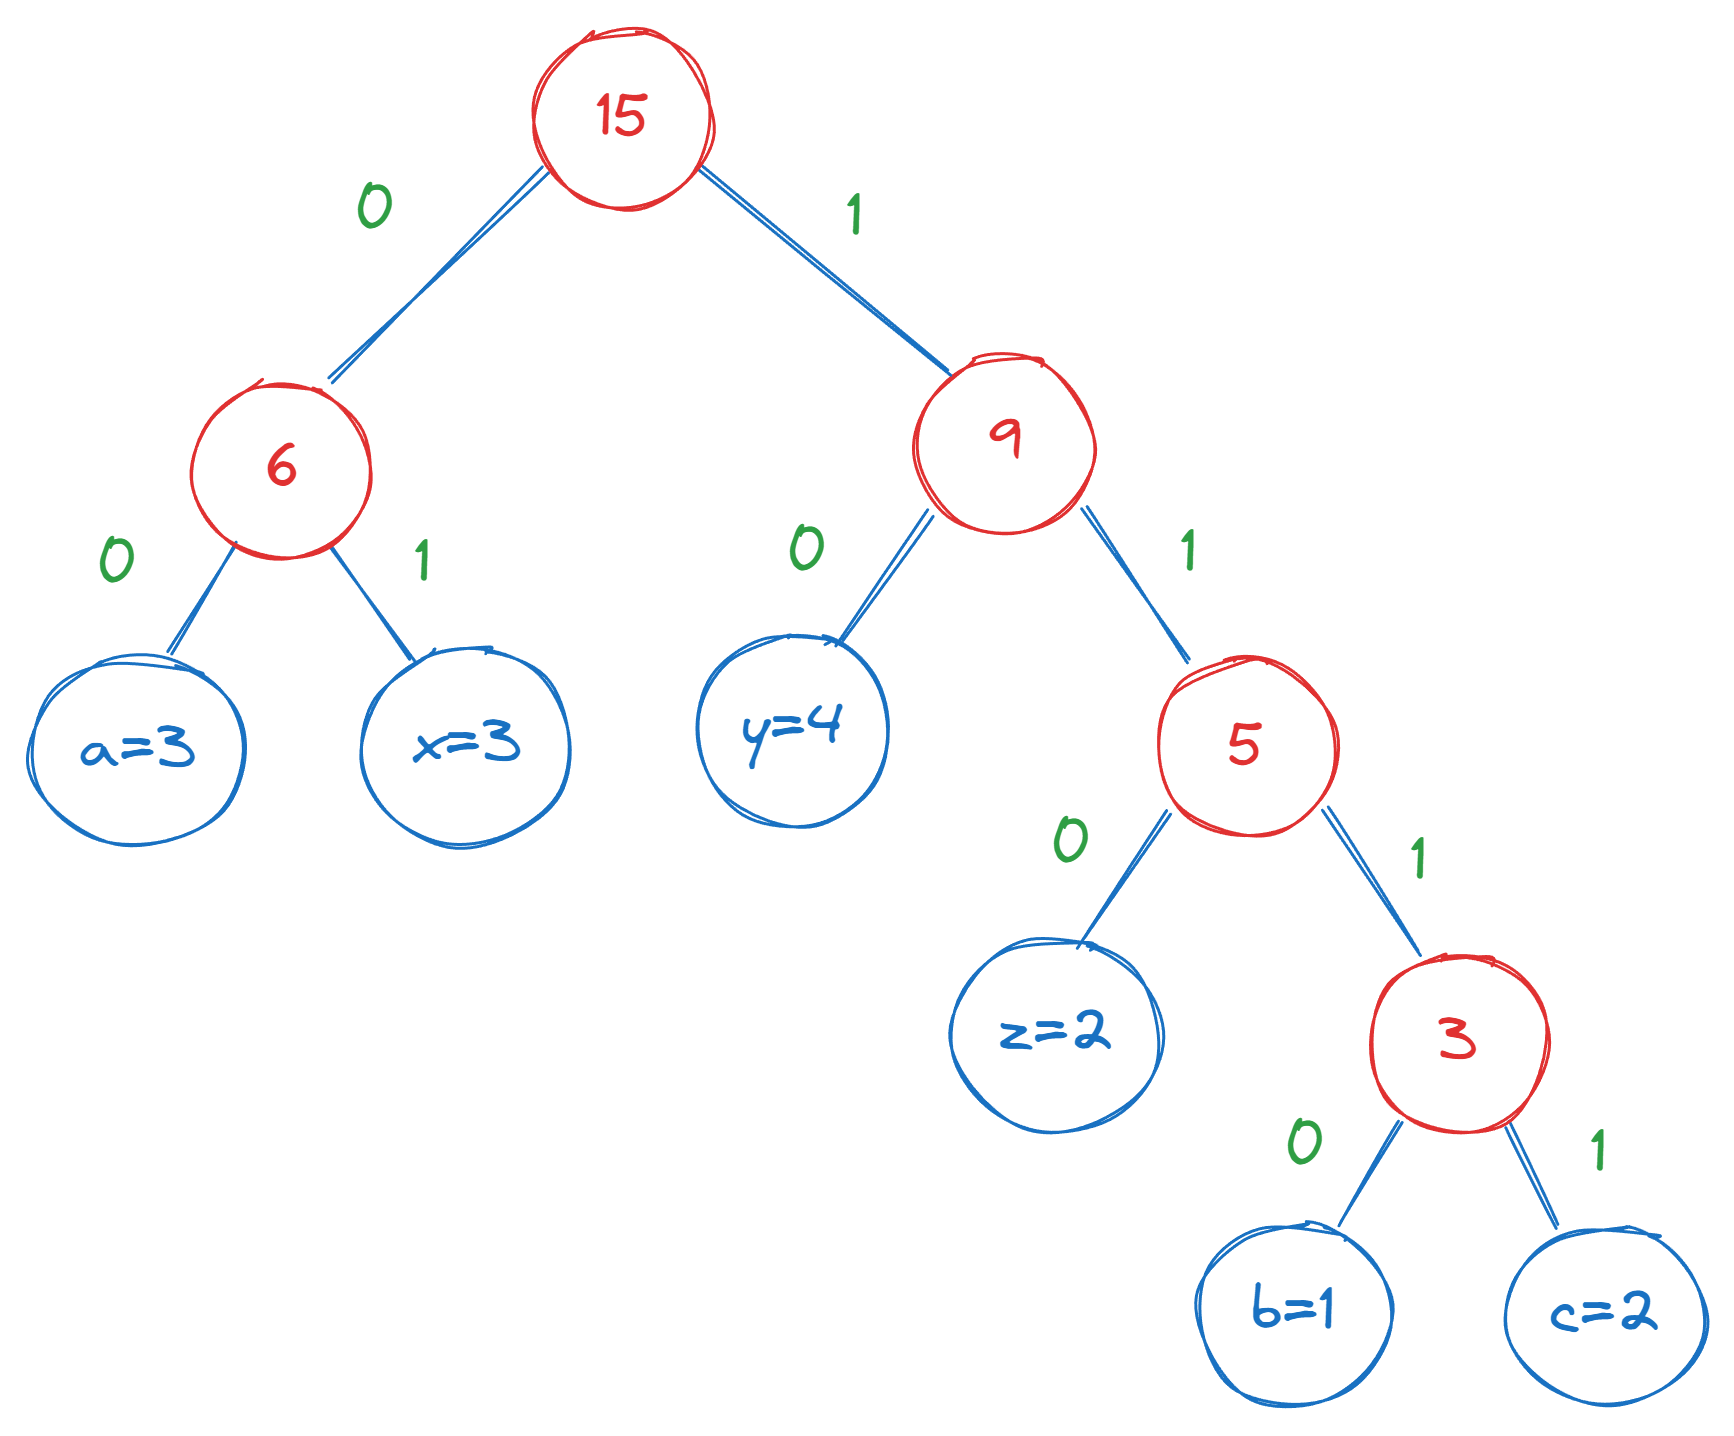
\includegraphics[width=0.65\linewidth]{HWs//HW11/figures/2.png}
\end{figure}
\\
Therefore, the Huffman codes for each character are
\begin{table}[!h]
    \centering
    \begin{tabular}{|c|c|c|c|c|c|}
        \hline
        b & c & z & a & x & y \\
        \hline
        1110 & 1111 & 110 & 00 & 01 & 10 \\
        \hline
    \end{tabular}
\end{table}
\\
In total, we need 
\[
    4 \times (1 + 2) + 3 \times 2 + 2 \times (3 + 3 + 4) = 38 ~\text{bits}
\]
to encode the message ``aaabccxxxyyyyzz”.
}